\subsection{Long term speckle pulsing}

In experiment, it is important to know the average speckle potential at the atoms. But unfortunately, it is hard to measure the power of the speckle beam directly at the atoms and infer the average speckle potential. Because in experiment, we can not put a power meter anywhere we want. After the closest point to the vacuum glass cell where we can use a power meter to measure the power. The beam goes through lenses, reflected by mirrors, glass cell or even dichroic mirrors. The power of the beam decreases at each of the optical component. To the best of our knowledge, for the previous experiments using speckle beams, the average speckle potential was not measured. It could be inferred by calculating the power given the power loss at each optical component is known. Or the power could be measured for an identical speckle beam set up on the test bench and assume the power at the atoms is the same for the speckle beam used in the experiment. 

Inspired by \cite{huckans2009quantum}, we think the average speckle potential can be measured by evolving the atoms under speckle beam pulses. Compared with \cite{huckans2009quantum}, for $t \gg t_{RN}$, we do not expect to see the collapse and revive phenomenon due to the anharmonicity of the speckle potential. Instead, the at long speckle pulsing time, the momentum distribution should reach equilibrium and by Virial theorem, the average stationary kinetic energy is half of the average total energy which is the initial average speckle potential. 

To confirm our understanding, we did numerical simulation of long-term speckle pulsing. Fig.~ \ref{fig:speckle_pulsing} show the simulation and experimental results of speckle pulsing for pulsing  duration up tp $2 {\rm ms}$. In the simulation, we release the BEC from the dipole trap and immediately turn on the speckle potential. The atoms evolve under the speckle potential and we keep track of the width of the momentum distribution. We did the simulation for different average speckle potential ranging from $0 {\rm Hz}$ to $1600 {\rm Hz}$, with $200 {\rm Hz}$ spacing. The results are shown as the nine curves, each one is averaged over 20 speckle realizations. When the average speckle potential is zero, the width of the momentum distribution increases driven by the mean-field expansion. From the simulation results shown in Fig.~ \ref{fig:speckle_pulsing}(a), the width of the momentum distribution increase rapidly evolving under speckle potential and becomes stationary after around $0.25 {\mu s}$. The stationary width increases with the average speckle potential. Fig.~\ref{fig:speckle_pulsing}(b) shows the experimental results. In experiment, we release the atoms from dipole trap, pulse speckle potential for up to $2 {\rm mm}$ followed by TOF. The time for speckle pulsing plus the time for TOF is fixed, $18 {\rm ms}$. We take absorption images after TOF and fit Gaussian function to the density profile of the atoms in the images. Fig.~\ref{fig:speckle_pulsing}(b) shows the with of the fitted Gaussian function vs speckle pulses duration. The Gaussian width increases with the pulsing duration in short-term and becomes stationary after around $0.25 {\rm ms}$, which is consistent with the simulation results. 


\begin{figure*}
    \centering
    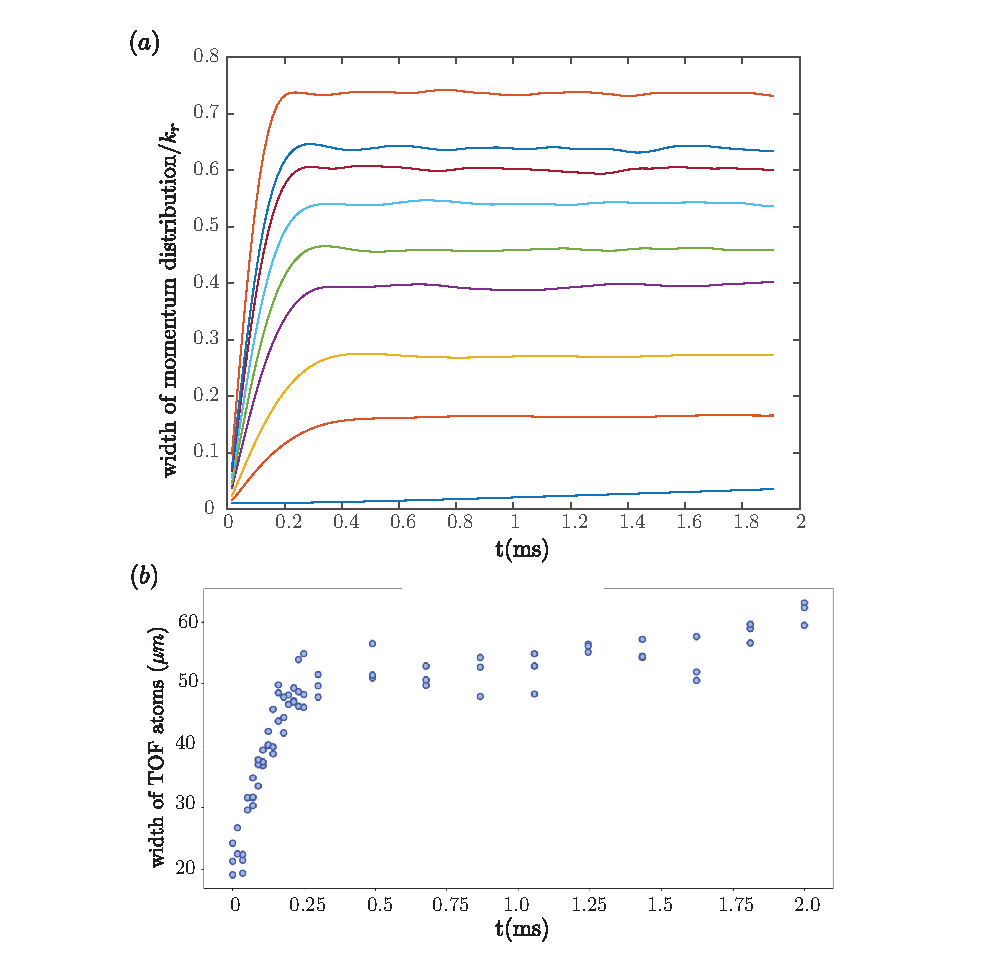
\includegraphics{Chapter6_secs/speckle_pulsing_width.pdf}
    \caption{Simulation and experiment of speckle beam pulsing. (a). Absorption images after TOF for different speckle pulsing time. The width of atoms increases as the speckle pulsing time increases from 0 to $\approx 2 {\rm ms}$. After which the width reaches equilibrium. (b). The Gaussian width of atoms in absorption images for  different speckle pulsing time.}
    \label{fig:speckle_pulsing}
\end{figure*}

Our experimental sequence start with a BEC held in a cross dipole trap. Immediately after turning off the dipole trap, we pulse the speckle beam for time $\tau$, followed by a time-of-flight (TOF). An absorption image is taken after the TOF. For the data we took, $\tau$ range from $0 {\rm ms}$ to $6 {\rm ms}$. The TOF maps the momentum distribution to the position distribution. So by analysing the optical depth of the images, we can get the momentum distribution of atoms after the speckle pulsing and compute its width from which, the average kinetic energy and average speckle potential depth can be estimated.

\begin{figure*}
    \centering
    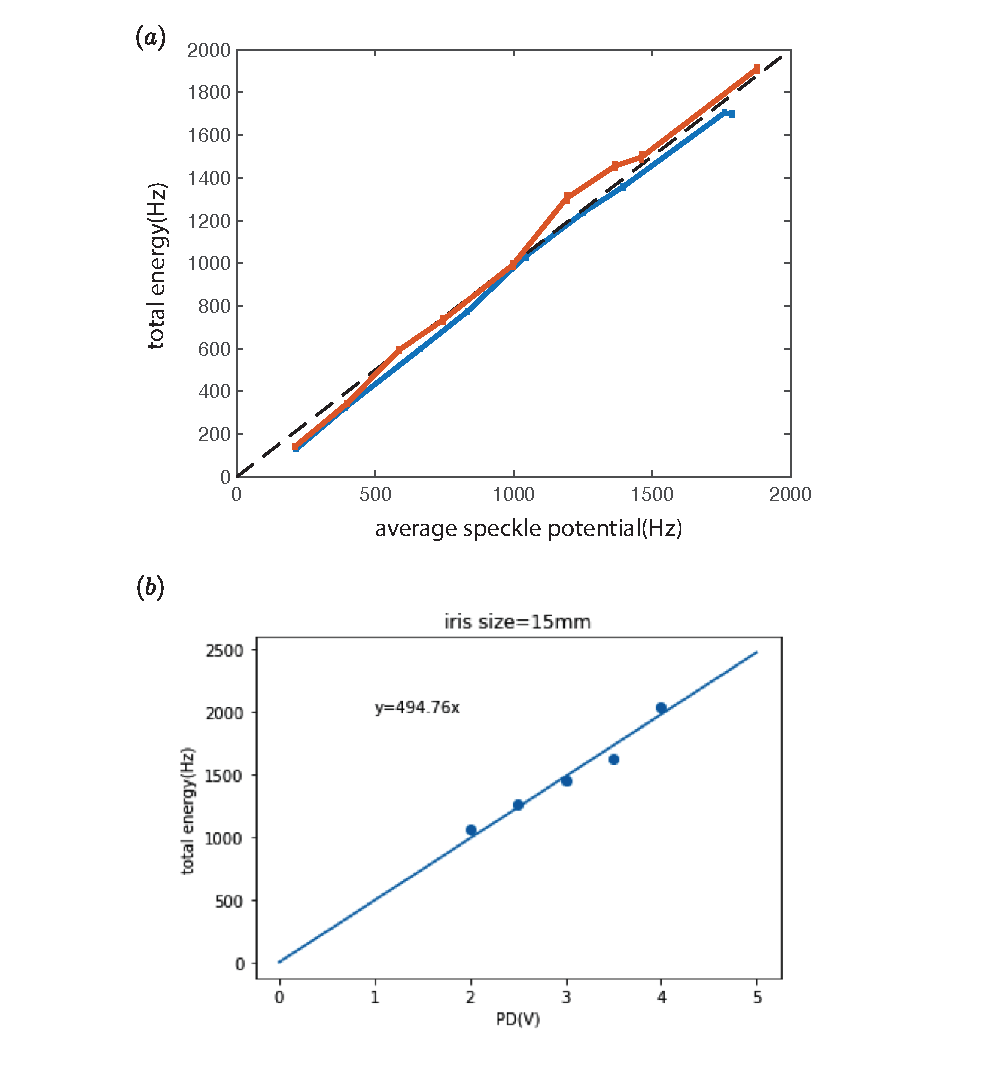
\includegraphics{Chapter6_secs/average_speckle_potential.pdf}
    \caption{s}
    \label{fig:avg_speckle_poten}
\end{figure*}




Fig.~(\ref{fig:speckle_pulsing}) shows absorption images and the fitted Gaussian width. With TOF, the momentum distribution of atoms after speckle pulsing is mapped to the distribution in space. So the optical depth of the absorption images is proportional to the momentum distribution before TOF. For short time speckle pulsing, the width of the momentum distribution increases rapidly. After $\approx 2 {\rm ms}$, the atoms reach equilibrium under speckle potential and the width of the momentum distribution reaches maximum. The average kinetic energy of the atoms can be calculated from the width of momentum distribution in equilibrium. And by Virial Theorem, the total energy can be calculated and compared with the average speckle potential depth. As Fig.~(\ref{fig:speckle_pulsing})(a) shows, we measure the photodiode reading which is proportional to the power of the speckle beam and the average speckle depth. We fit a line crossing the origin so the average speckle potential can be inferred by the photodiode reading directly.

As our model shows, in short time speckle pulsing, the momentum distribution should be proportional to the speckle potential PSD except for the peak at $k=0$. In Fig.~(\ref{fig:speckle_pulsing})(b), we compute the average momentum distribution in short time for different iris size, with the central peak masked. As iris size changes, the cutoff of the PSD changes and in theory should be measurable by comparing the masked normalized momentum distribution. We measured the momentum distribution for two iris sizes,  $6.5 {\rm mm}$ and $15 {\rm mm}$. In theory, the $k_c$ of the PSD should be $1.3 \kr$ and $1.9 \kr$, respectively. But in our measurement, the difference is not clear due to the noise of our measurement.
